\documentclass[12pt, varwidth, border=5mm]{standalone}
\usepackage{tikz}
\usepackage{amsmath}
% Underlining package
\usepackage{ulem}
\usetikzlibrary{calc}
\usetikzlibrary{angles,quotes}
% \usepackage[a4paper, portrait, margin=1cm]{geometry}

\begin{document}
\section*{ }
    \begin{minipage}{0.55\textwidth}
  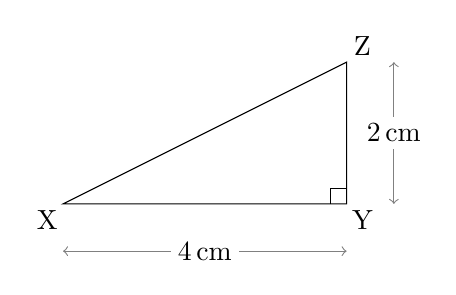
\begin{tikzpicture}[scale=1.0, baseline=(current bounding box.north)]
    \begin{scope}[rotate=0]
        % Draw

        \draw (0,0) coordinate (X) --
         ++(3.602,0) coordinate (Y) --
         ++(90:1.801) coordinate (Z) -- cycle;

        \pic [draw, -, angle radius=0.2cm] {right angle=Z--Y--X};

        % Vertex LABELS
        % Labels relative to shape geometry
        \node at ($(X)+(-0.2,-0.2)$) {X};
        \node at ($(Y)+(0.2,-0.2)$) {Y};
        \node at ($(Z)+(0.2,0.2)$) {Z};


        % dotted/dashed arrows shifted away from edges
        % Horizontal side (A-B), shifted down
        \draw[<->, gray]
            ($(X) + (0,-0.6cm)$) -- ($(Y) + (0,-0.6cm)$)
            node[black, midway, fill=white, inner sep=2.5pt] {4\,cm};

        % Vertical side (B-C), shifted right
        \draw[<->, gray]
            ($(Y) + (0.6cm,0)$) -- ($(Z) + (0.6cm,0)$)
            node[black, midway, fill=white, xshift=0mm, inner sep=2.5pt] {2\,cm};

    \end{scope}
\end{tikzpicture}
\end{minipage}%
\hfill
\begin{minipage}{.4\textwidth}
  \begin{align*}
    \text{Area} &= \frac{1}{2} \text{bh} \\
    \text{Area} &= \frac{1}{2} \times 4 \text{cm} \times 2 \text{cm}  \\
    \text{Area} &= 4.0 \text{cm}^2
  \end{align*}
\end{minipage}

\end{document}
